% Options for packages loaded elsewhere
\PassOptionsToPackage{unicode}{hyperref}
\PassOptionsToPackage{hyphens}{url}
\PassOptionsToPackage{dvipsnames,svgnames,x11names}{xcolor}
%
\documentclass[
]{article}
\title{Usage code for data repository

Building age map, Vienna, around 1920}
\author{Ulrich Kral, Ferdinand Reimer}
\date{}

\usepackage{amsmath,amssymb}
\usepackage{lmodern}
\usepackage{iftex}
\ifPDFTeX
  \usepackage[T1]{fontenc}
  \usepackage[utf8]{inputenc}
  \usepackage{textcomp} % provide euro and other symbols
\else % if luatex or xetex
  \usepackage{unicode-math}
  \defaultfontfeatures{Scale=MatchLowercase}
  \defaultfontfeatures[\rmfamily]{Ligatures=TeX,Scale=1}
\fi
% Use upquote if available, for straight quotes in verbatim environments
\IfFileExists{upquote.sty}{\usepackage{upquote}}{}
\IfFileExists{microtype.sty}{% use microtype if available
  \usepackage[]{microtype}
  \UseMicrotypeSet[protrusion]{basicmath} % disable protrusion for tt fonts
}{}
\makeatletter
\@ifundefined{KOMAClassName}{% if non-KOMA class
  \IfFileExists{parskip.sty}{%
    \usepackage{parskip}
  }{% else
    \setlength{\parindent}{0pt}
    \setlength{\parskip}{6pt plus 2pt minus 1pt}}
}{% if KOMA class
  \KOMAoptions{parskip=half}}
\makeatother
\usepackage{xcolor}
\IfFileExists{xurl.sty}{\usepackage{xurl}}{} % add URL line breaks if available
\IfFileExists{bookmark.sty}{\usepackage{bookmark}}{\usepackage{hyperref}}
\hypersetup{
  pdfauthor={Ulrich Kral, Ferdinand Reimer},
  colorlinks=true,
  linkcolor={Maroon},
  filecolor={Maroon},
  citecolor={Blue},
  urlcolor={blue},
  pdfcreator={LaTeX via pandoc}}
\urlstyle{same} % disable monospaced font for URLs
\usepackage[margin=1in]{geometry}
\usepackage{graphicx}
\makeatletter
\def\maxwidth{\ifdim\Gin@nat@width>\linewidth\linewidth\else\Gin@nat@width\fi}
\def\maxheight{\ifdim\Gin@nat@height>\textheight\textheight\else\Gin@nat@height\fi}
\makeatother
% Scale images if necessary, so that they will not overflow the page
% margins by default, and it is still possible to overwrite the defaults
% using explicit options in \includegraphics[width, height, ...]{}
\setkeys{Gin}{width=\maxwidth,height=\maxheight,keepaspectratio}
% Set default figure placement to htbp
\makeatletter
\def\fps@figure{htbp}
\makeatother
\setlength{\emergencystretch}{3em} % prevent overfull lines
\providecommand{\tightlist}{%
  \setlength{\itemsep}{0pt}\setlength{\parskip}{0pt}}
\setcounter{secnumdepth}{5}
\usepackage{booktabs}
\usepackage{longtable}
\usepackage{array}
\usepackage{multirow}
\usepackage{wrapfig}
\usepackage{float}
\usepackage{colortbl}
\usepackage{pdflscape}
\usepackage{tabu}
\usepackage{threeparttable}
\usepackage{threeparttablex}
\usepackage[normalem]{ulem}
\usepackage{makecell}
\usepackage{xcolor}
\ifLuaTeX
  \usepackage{selnolig}  % disable illegal ligatures
\fi

\begin{document}
\maketitle

{
\hypersetup{linkcolor=}
\setcounter{tocdepth}{2}
\tableofcontents
}
\hypertarget{preface}{%
\section*{Preface}\label{preface}}
\addcontentsline{toc}{section}{Preface}

\textbf{This usage code}

\begin{itemize}
\item
  \textbf{is part} of the GitHub repository
  \href{https://github.com/ukral/building.map_1920}{building.map\_1920}.
  Check out the
  \href{https://github.com/ukral/building.map_1920/blob/main/README.md}{readme
  file} to learn more about the corresponding datasets and how to use
  and re-use the underlying R Markdown file.
\item
  \textbf{supplements} the paper ``Data description of `Building age map
  of Vienna and its surroundings around 1920'\,'', which is currently
  under review in
  \href{https://www.journals.elsevier.com/data-in-brief}{Data in Brief}.
\item
  \textbf{is for users} of the datasets who want to use and re-use the
  datasets.
\end{itemize}

\hypertarget{introduction-figures}{%
\section{Introduction figures}\label{introduction-figures}}

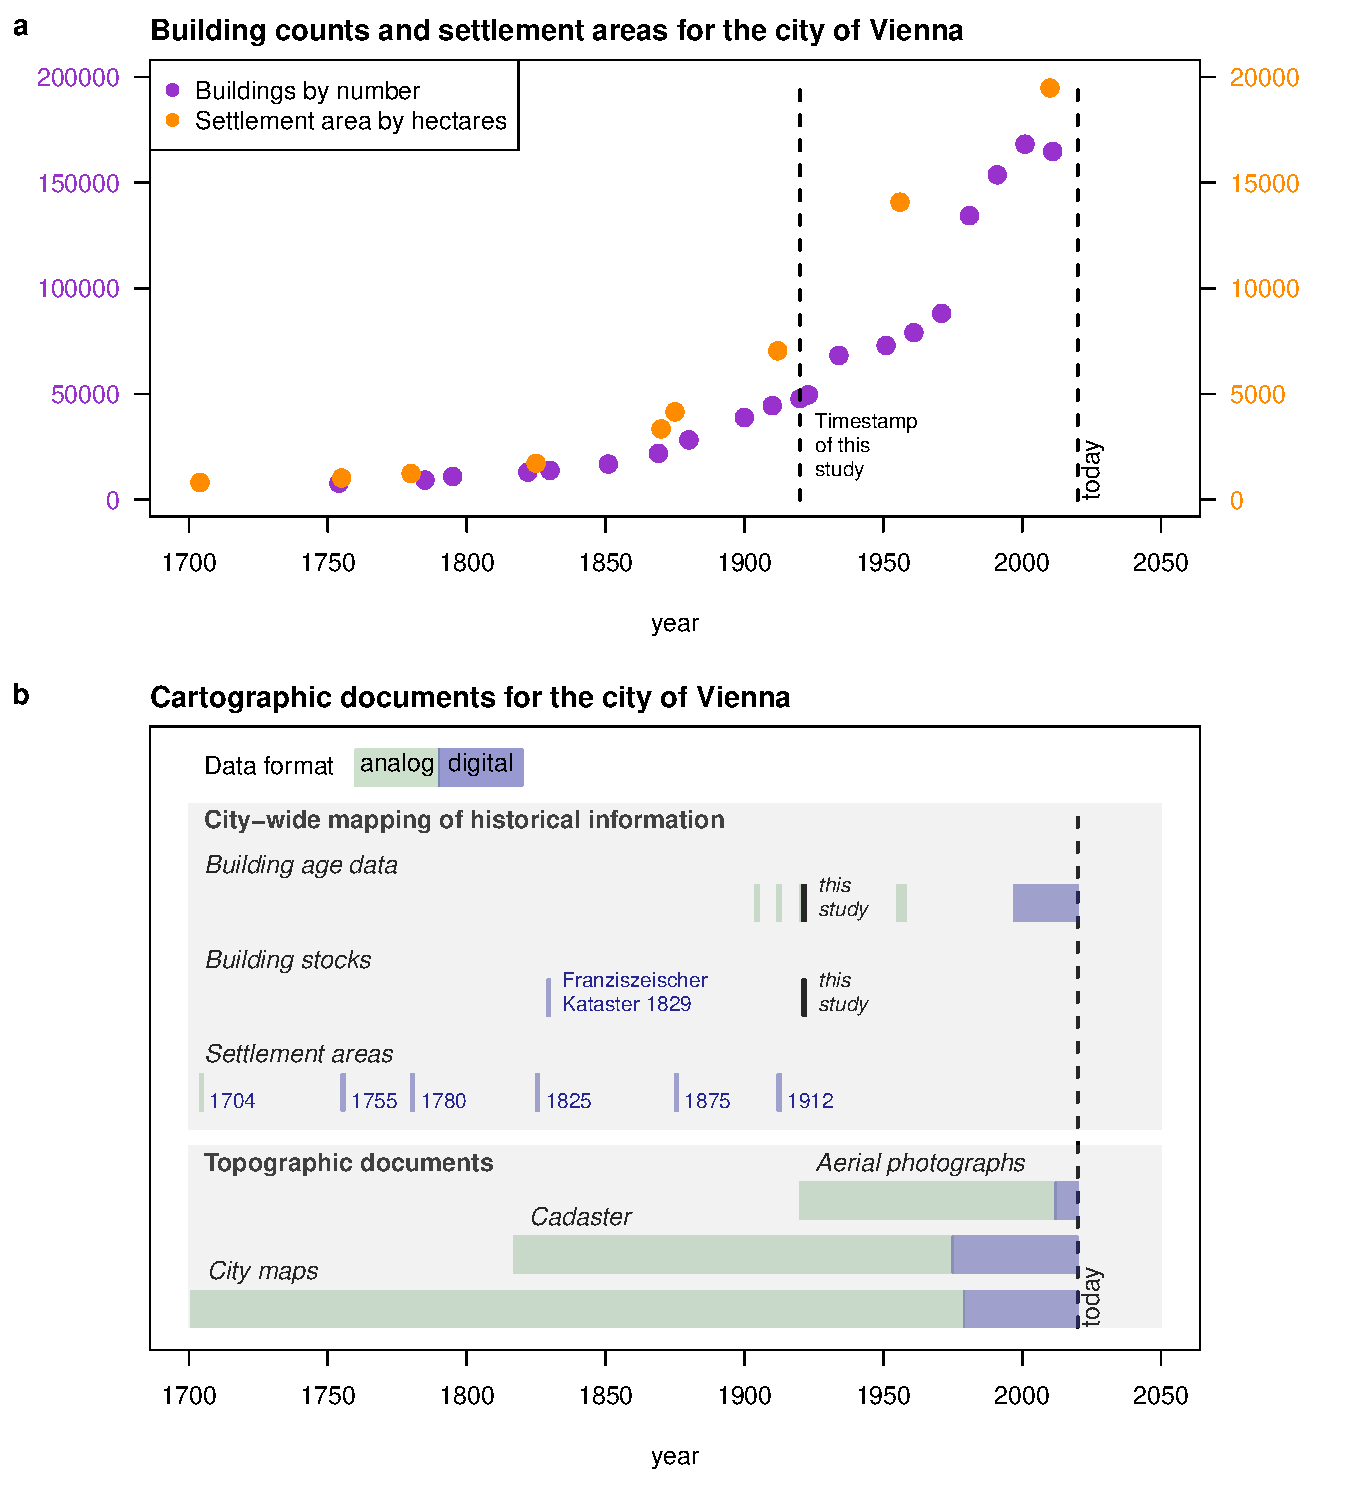
\includegraphics{Usage_code_files/figure-latex/unnamed-chunk-2-1.pdf}

\hypertarget{scales-of-analog-map-sheets}{%
\section{Scales of analog map
sheets}\label{scales-of-analog-map-sheets}}

Scales of building stock maps, which were used to retrieve the building
footprints: 1:NA, 1:5000, 1:3500, 1:1440, 1:10000, 1:2880. Note: NA
stands for ``not available'', because the digitial city map is
vectorized and therefore doesn't have a scale.

\hypertarget{addresss-changes}{%
\section{Addresss changes}\label{addresss-changes}}

Address changes between `Address.2019' and `Address.1920'. Scope:
`Address\_review' = yes

\begin{tabular}[t]{l|r|r}
\hline
address change & affected polygons & ratio [\%]\\
\hline
yes & 13,108 & 26\\
\hline
no & 36,478 & 74\\
\hline
\end{tabular}

\hypertarget{area-of-building-footprints}{%
\section{Area of building
footprints}\label{area-of-building-footprints}}

The ``Area'' records are summarized by ``UD.1920'' and ``UD.2020'',
respectively, and plotted in the next figure.

\begin{verbatim}
## Warning: Removed 2 rows containing missing values (geom_bar).
\end{verbatim}

\begin{verbatim}
## Warning: Removed 2 rows containing missing values (geom_text).
\end{verbatim}

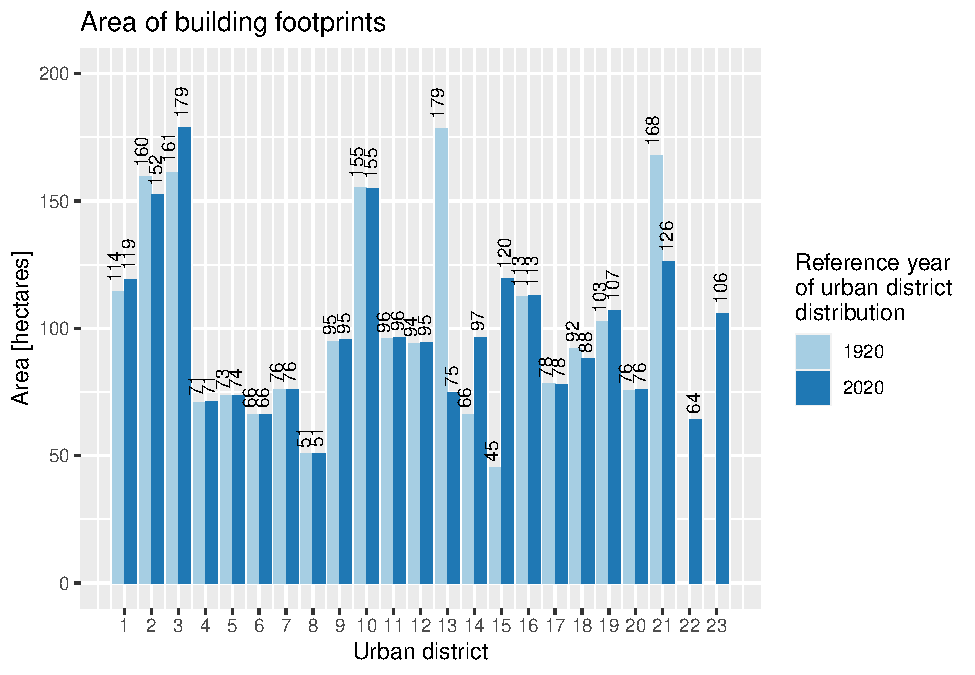
\includegraphics{Usage_code_files/figure-latex/unnamed-chunk-4-1.pdf}

\hypertarget{data-sources-to-retrieve-building-footprints}{%
\section{Data sources to retrieve building
footprints}\label{data-sources-to-retrieve-building-footprints}}

The ``Polygon.source\_name'' records were grouped by ``UD.2020'',
summarized by ``Area'' and plotted in the next figure.

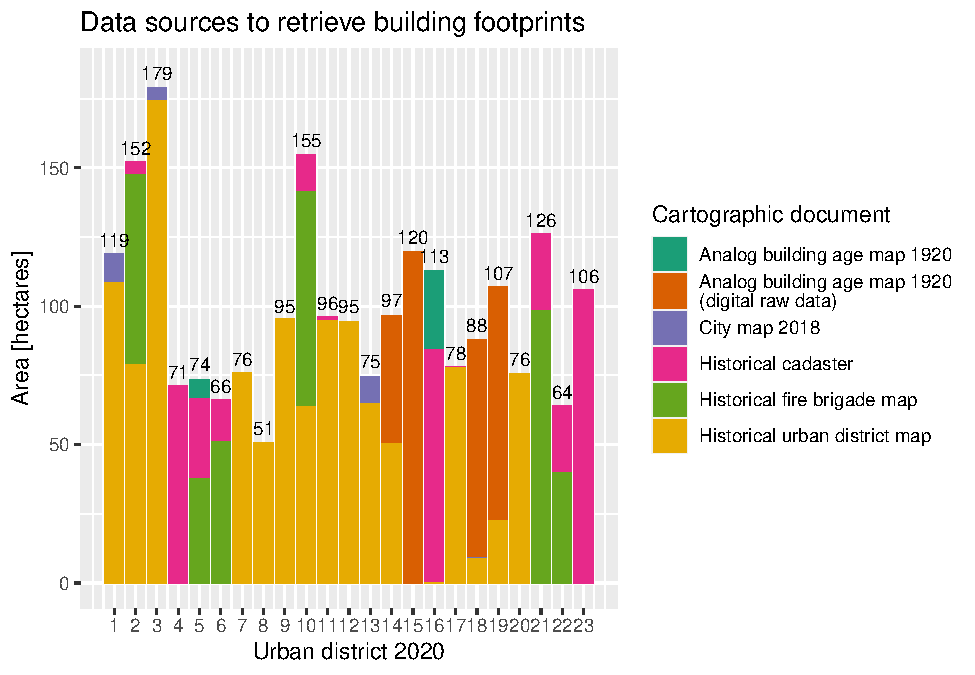
\includegraphics{Usage_code_files/figure-latex/unnamed-chunk-5-1.pdf}

\begin{itemize}
\tightlist
\item
  Number of unique maps sheets: 134. Retrieved from City map 2018,
  Historical urban district map, Historical fire brigade map, Historical
  cadaster, Analog building age map 1920, Analog building age map 1920
  (digital raw data).
\item
  Number of unique timestamps: 19.
\end{itemize}

\hypertarget{editors-of-vectorized-building-footprints}{%
\section{Editors of vectorized building
footprints}\label{editors-of-vectorized-building-footprints}}

The ``Editor'' records were grouped by ``UD.2020'', summarized by
``Area'' and plotted in the next figure.

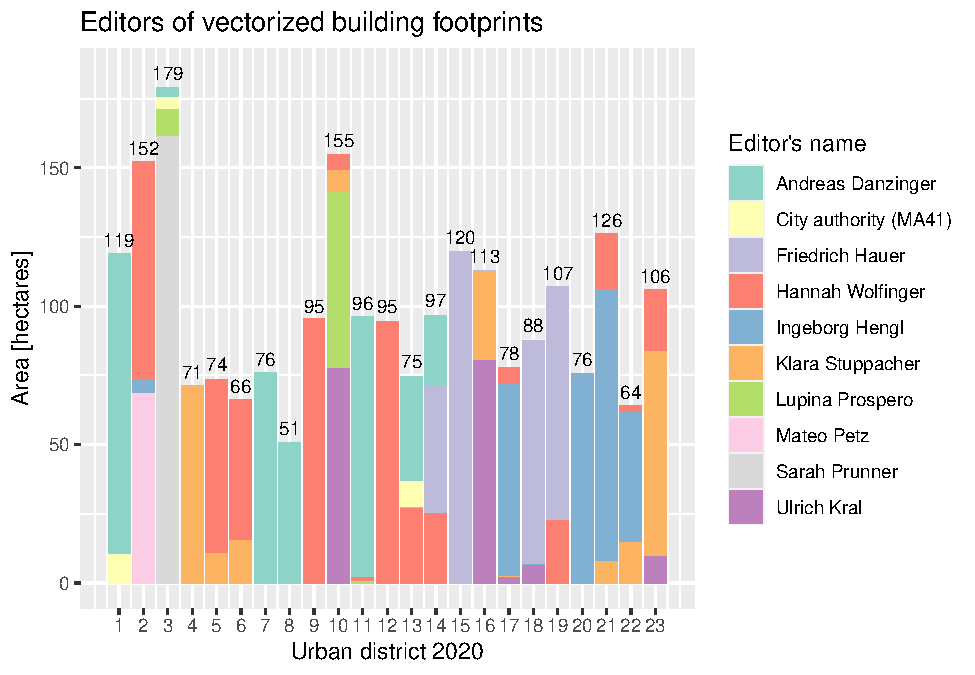
\includegraphics{Usage_code_files/figure-latex/unnamed-chunk-6-1.pdf}

\begin{itemize}
\tightlist
\item
  Number of unique editors: 10.
\end{itemize}

\hypertarget{temporal-presence-of-building-footprints}{%
\section{Temporal presence of building
footprints}\label{temporal-presence-of-building-footprints}}

The ``TP\_pub.date\_period'' records were grouped by ``UD.2020'',
summarized by ``Area'' and plotted in the next figure.

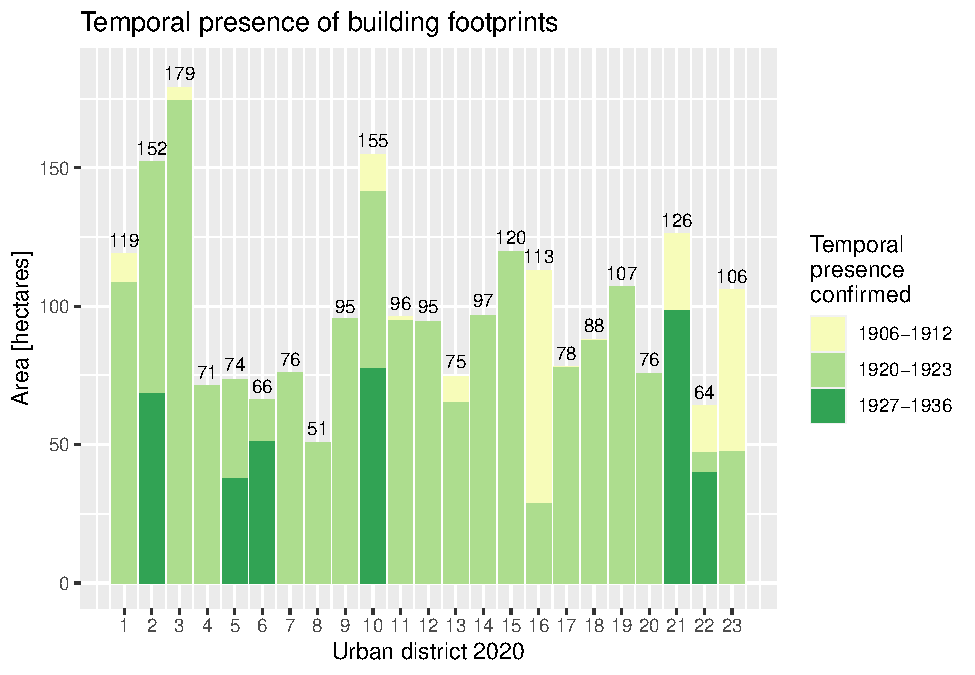
\includegraphics{Usage_code_files/figure-latex/unnamed-chunk-7-1.pdf}

\begin{itemize}
\tightlist
\item
  City-wide data grouped into 3 periods.

  \begin{tabular}[t]{l|r|r}
  \hline
  TP\_pub.date\_period & sum\_area\_abs & sum\_area\_rel\\
  \hline
  1906-1912 & 227 & 10\\
  \hline
  1920-1923 & 1,679 & 74\\
  \hline
  1927-1936 & 373 & 16\\
  \hline
  \end{tabular}
\end{itemize}

\hypertarget{period-of-constrution}{%
\section{Period of constrution}\label{period-of-constrution}}

The ``PoC'' records were grouped by two different types of timespan,
summarized by ``Area'' and plotted in the next figure.

\begin{verbatim}
## [1] CD.bs   min     max     szbg_bp
## <0 Zeilen> (oder row.names mit Länge 0)
\end{verbatim}

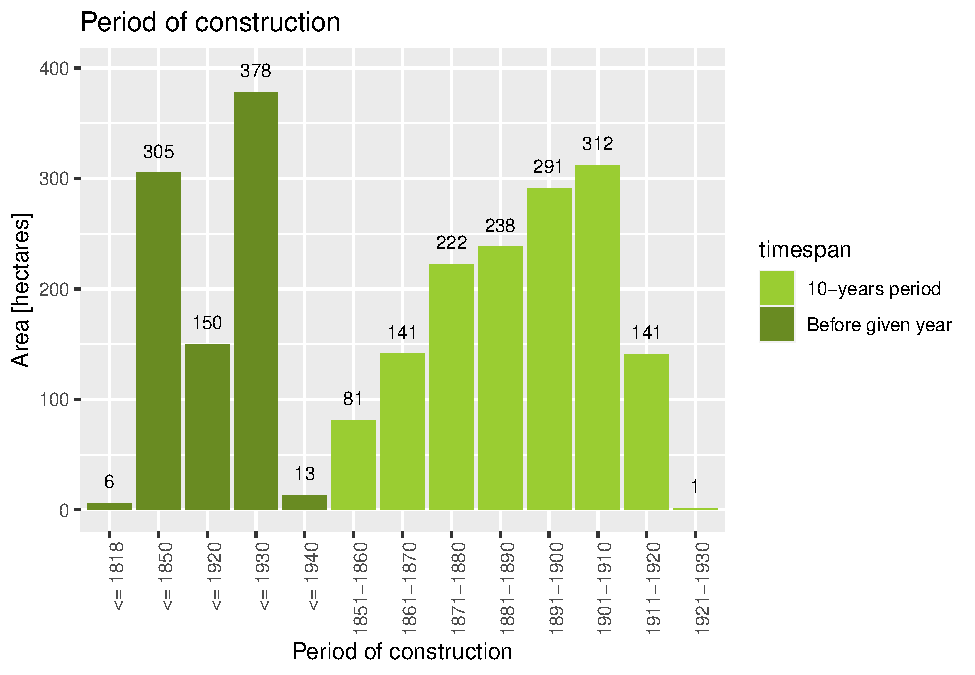
\includegraphics{Usage_code_files/figure-latex/unnamed-chunk-8-1.pdf}

\begin{itemize}
\tightlist
\item
  Summary: Assignment of construction dates.

  \begin{tabular}[t]{l|r|r|r}
  \hline
  Data field & N of assigments & Unique dates before h & Unique dates after h\\
  \hline
  CD.abam & 49,156 & 12 & 10\\
  \hline
  CD.bs & 3,125 & 238 & 12\\
  \hline
  TP\_pub.date\_year & 28,359 & 19 & 3\\
  \hline
  \end{tabular}
\item
  Summary: Grouping PoC records.

  \begin{tabular}[t]{l|r|r}
  \hline
  timespan & sum\_area & sum\_area\_rel\\
  \hline
  10-years period & 1,428 & 63\\
  \hline
  Before given year & 851 & 37\\
  \hline
  \end{tabular}
\item
  Number of construction date assignments.

  \begin{tabular}[t]{r|r|r}
  \hline
  CD\_multiple & count\_CD\_multiple & count\_CD\_multiple\_rel\\
  \hline
  1 & 28,359 & 35\\
  \hline
  2 & 35,233 & 44\\
  \hline
  3 & 17,048 & 21\\
  \hline
  \end{tabular}
\end{itemize}

\hypertarget{data-sources-to-retrieve-building-construction-dates}{%
\section{Data sources to retrieve building construction
dates}\label{data-sources-to-retrieve-building-construction-dates}}

The ``PoC.source\_name'' records were grouped by ``UD.2020'', summarized
by ``Area'' and plotted in the next figure.

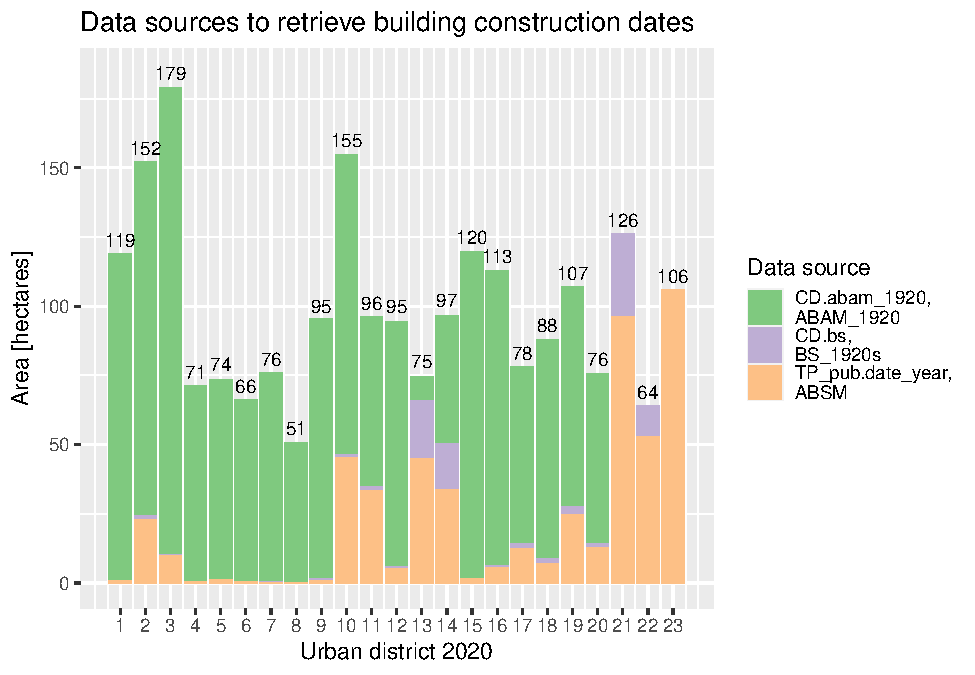
\includegraphics{Usage_code_files/figure-latex/unnamed-chunk-9-1.pdf}

\begin{itemize}
\tightlist
\item
  City-wide data:

  \begin{tabular}[t]{l|r|r}
  \hline
  PoC.source\_name & sum\_area & sum\_area\_rel\\
  \hline
  CD.abam\_1920,
  ABAM\_1920 & 1,665 & 73\\
  \hline
  CD.bs,
  BS\_1920s & 94 & 4\\
  \hline
  TP\_pub.date\_year,
  ABSM & 520 & 23\\
  \hline
  \end{tabular}
\end{itemize}

\hypertarget{location-of-building-footprints-within-city-limits-1920}{%
\section{Location of building footprints within city limits
1920}\label{location-of-building-footprints-within-city-limits-1920}}

The ``Location.city\_limits\_1920'' records were grouped by ``UD.2020'',
summarized by ``Area'' and plotted in the next figure.

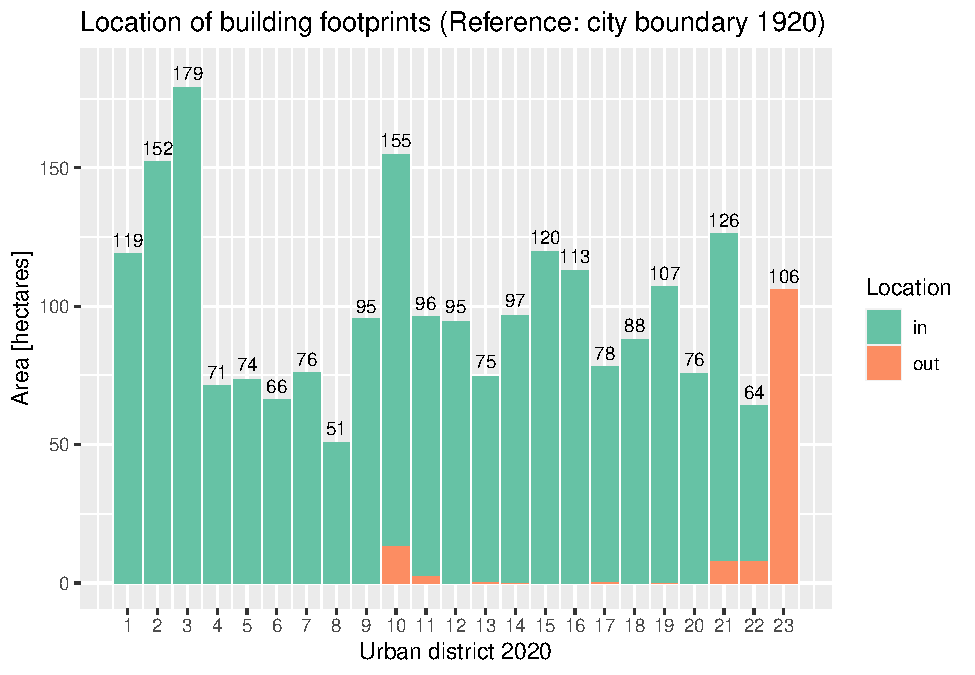
\includegraphics{Usage_code_files/figure-latex/unnamed-chunk-10-1.pdf}

\begin{itemize}
\tightlist
\item
  City-wide data:

  \begin{tabular}[t]{l|r|r}
  \hline
  Location.city\_limit\_1920 & sum\_area & sum\_area\_rel\\
  \hline
  in & 2,142 & 94\\
  \hline
  out & 137 & 6\\
  \hline
  \end{tabular}
\end{itemize}

\hypertarget{location-of-building-footprints-within-scope-of-analog-building-age-map-1920}{%
\section{Location of building footprints within scope of analog building
age map
1920}\label{location-of-building-footprints-within-scope-of-analog-building-age-map-1920}}

The ``Location.ABAM\_1920'' records were grouped by ``UD.2020'',
summarized by ``Area'' and plotted in the next figure.

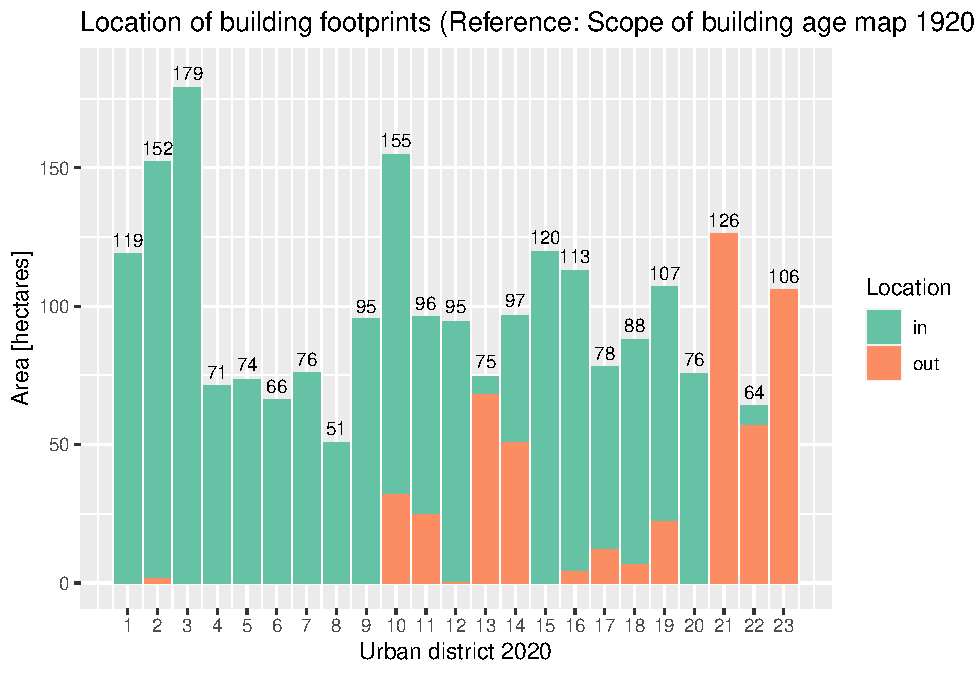
\includegraphics{Usage_code_files/figure-latex/unnamed-chunk-11-1.pdf}

\begin{itemize}
\tightlist
\item
  City-wide data:

  \begin{tabular}[t]{l|r|r}
  \hline
  Location.abam\_1920 & sum\_area & sum\_area\_rel\\
  \hline
  in & 1,767 & 78\\
  \hline
  out & 512 & 22\\
  \hline
  \end{tabular}
\end{itemize}

\hypertarget{building-counts-by-urban-district}{%
\section{Building counts by urban
district}\label{building-counts-by-urban-district}}

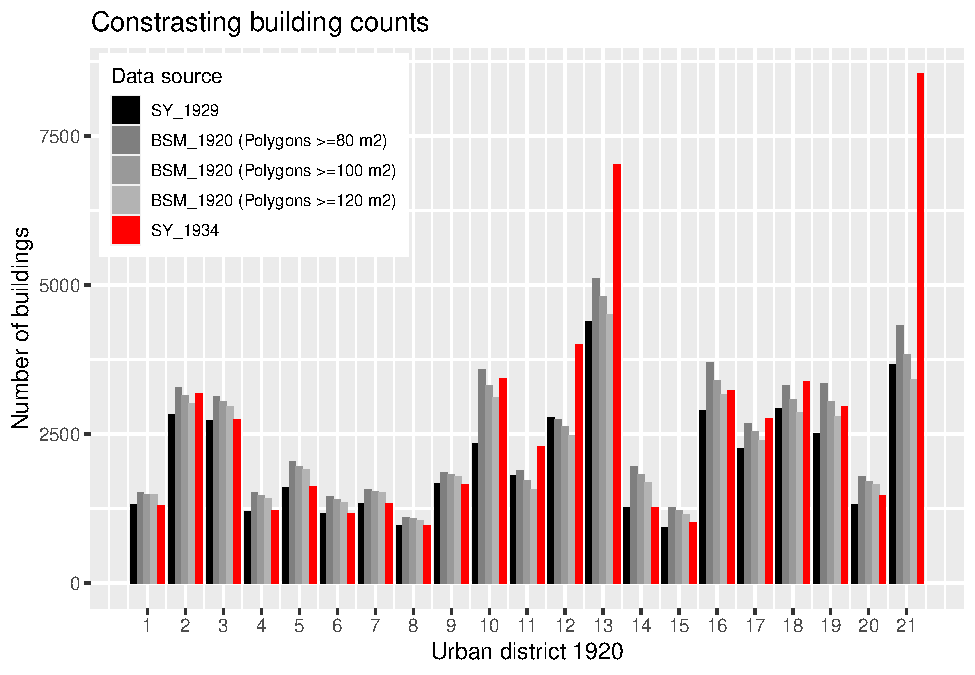
\includegraphics{Usage_code_files/figure-latex/unnamed-chunk-12-1.pdf}

\hypertarget{building-footprint-presence-in-1920}{%
\section{Building footprint presence in
1920}\label{building-footprint-presence-in-1920}}

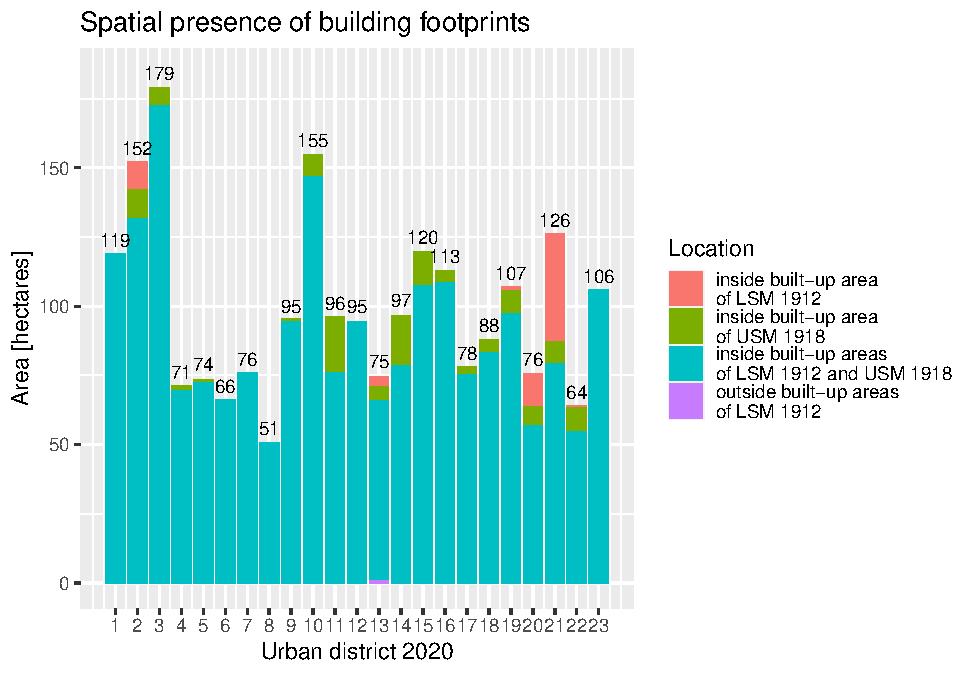
\includegraphics{Usage_code_files/figure-latex/unnamed-chunk-13-1.pdf}
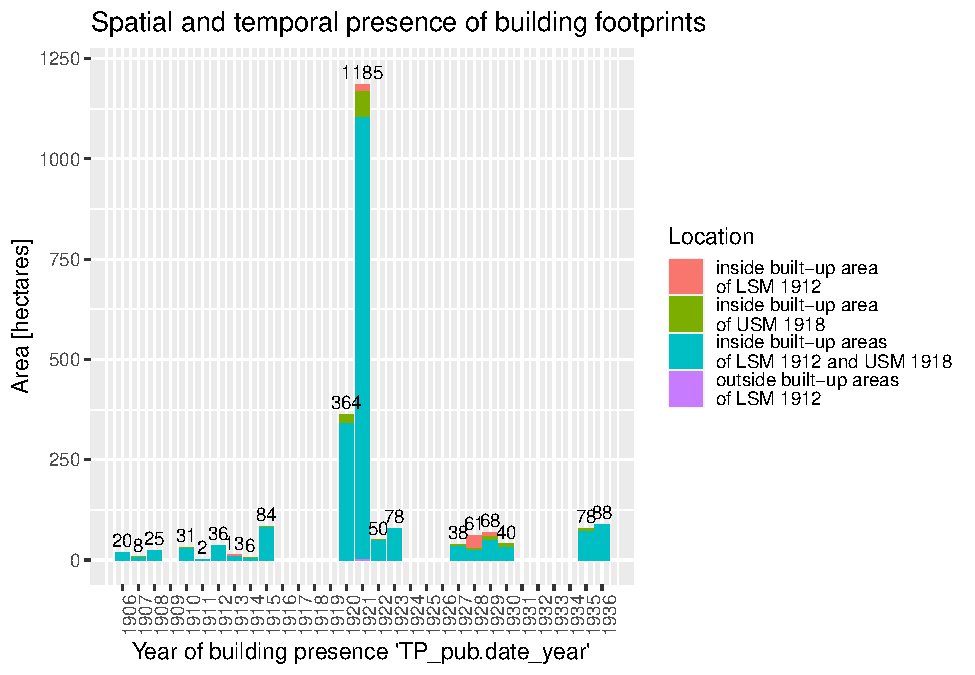
\includegraphics{Usage_code_files/figure-latex/unnamed-chunk-13-2.pdf}

\begin{itemize}
\tightlist
\item
  City-wide data:

  \begin{tabular}[t]{l|r|r}
  \hline
  Presence.conf & sum\_area & sum\_area\_rel\\
  \hline
  inside built-up area
  of LSM 1912 & 68 & 3\\
  \hline
  inside built-up area
  of USM 1918 & 127 & 6\\
  \hline
  inside built-up areas
  of LSM 1912 and USM 1918 & 2,083 & 91\\
  \hline
  outside built-up areas
  of LSM 1912 & 1 & 0\\
  \hline
  \end{tabular}
\end{itemize}

\hypertarget{construction-years}{%
\section{Construction years}\label{construction-years}}

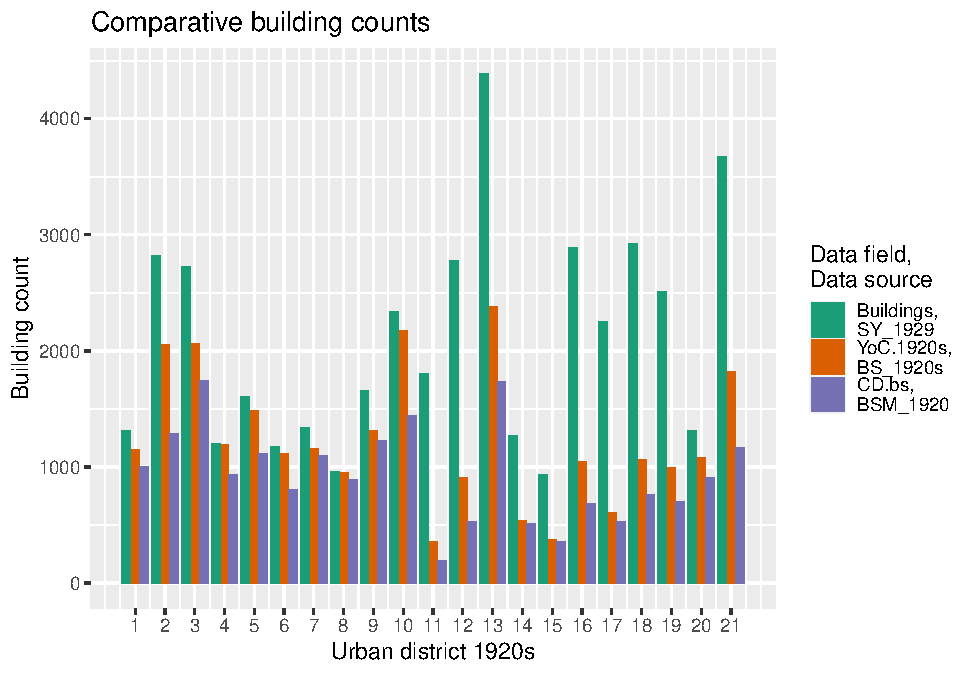
\includegraphics{Usage_code_files/figure-latex/unnamed-chunk-14-1.pdf}
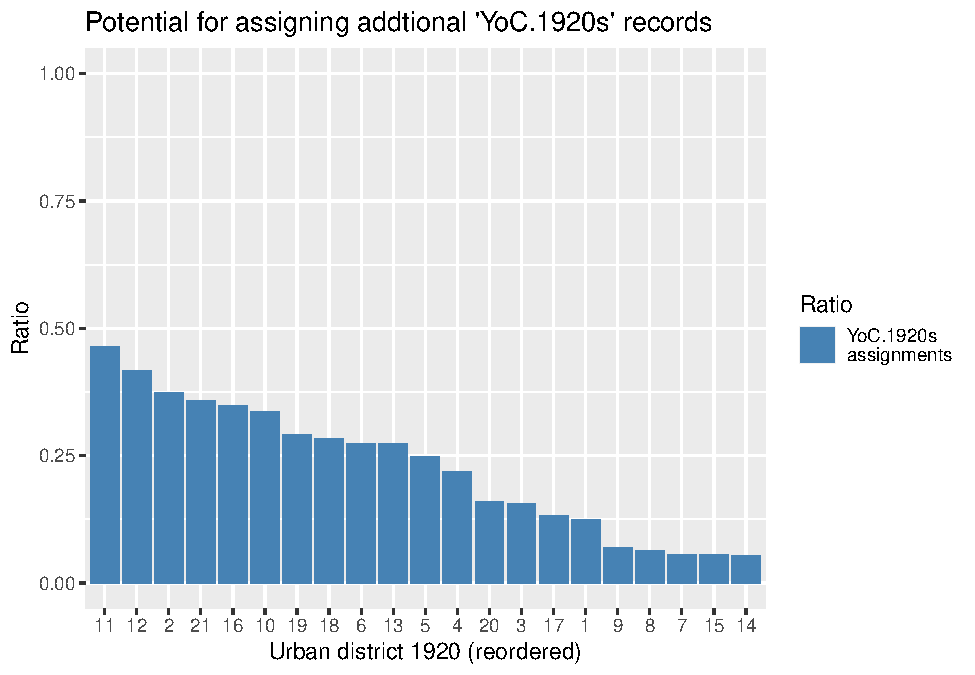
\includegraphics{Usage_code_files/figure-latex/unnamed-chunk-14-2.pdf}

\begin{itemize}
\item
  BS\_1920s perspective: : The BS\_1920s includes
  \ensuremath{2.5859\times 10^{4}}(100\%) entries with records in
  ``YoC.1920'', ``STR.1920s'' and ``BN.1920''. The latter two are needed
  to join the BS\_1920s and BSM\_1920. The workflow in this study
  captured \ensuremath{1.9631\times 10^{4}} (76\%) ``YoC.1920s'' records
  and assigned them to buildings in BSM\_1920. In other words, the
  remaining potential for assignments is (24\%).
\item
  Statistical yearbook (SY\_1929) perspective:

  \begin{tabular}[t]{l|r|r}
  \hline
  data\_source & count & ratio\\
  \hline
  CD.bs\_BSM\_1920 & 19,631 & 45\\
  \hline
  SY\_1929 & 43,910 & 100\\
  \hline
  YoC.1920s\_BS\_1920s & 25,859 & 59\\
  \hline
  \end{tabular}
\end{itemize}

\hypertarget{construction-periods}{%
\section{Construction periods}\label{construction-periods}}

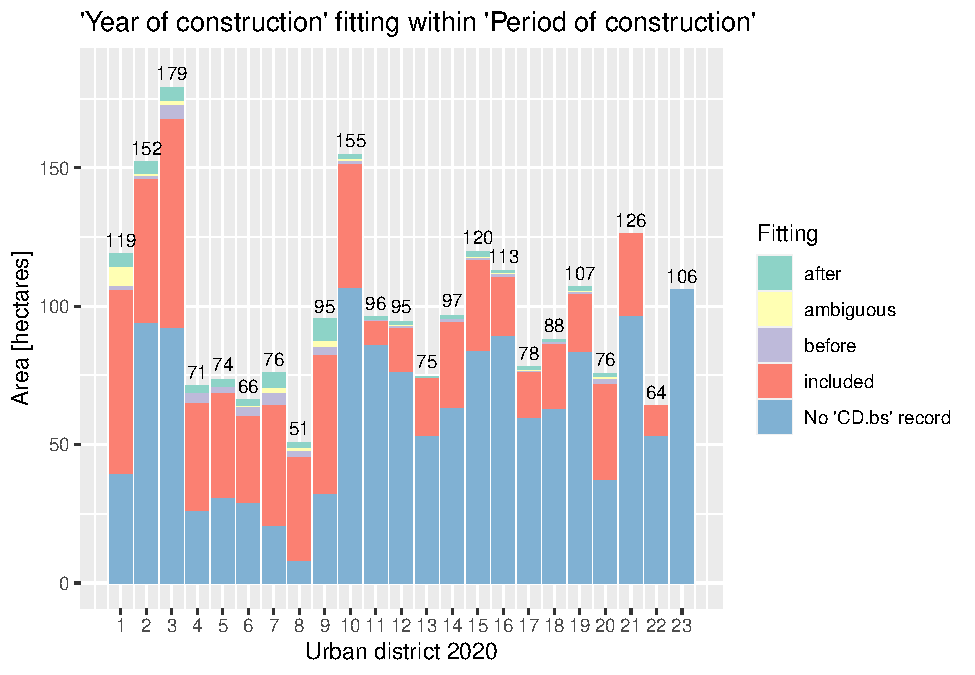
\includegraphics{Usage_code_files/figure-latex/unnamed-chunk-15-1.pdf}
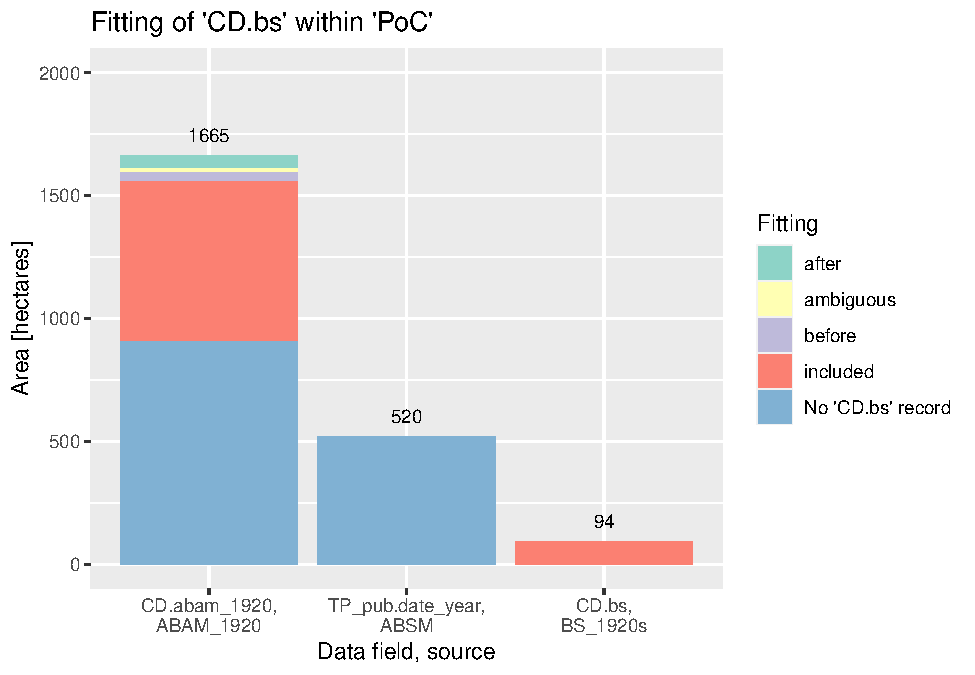
\includegraphics{Usage_code_files/figure-latex/unnamed-chunk-15-2.pdf}
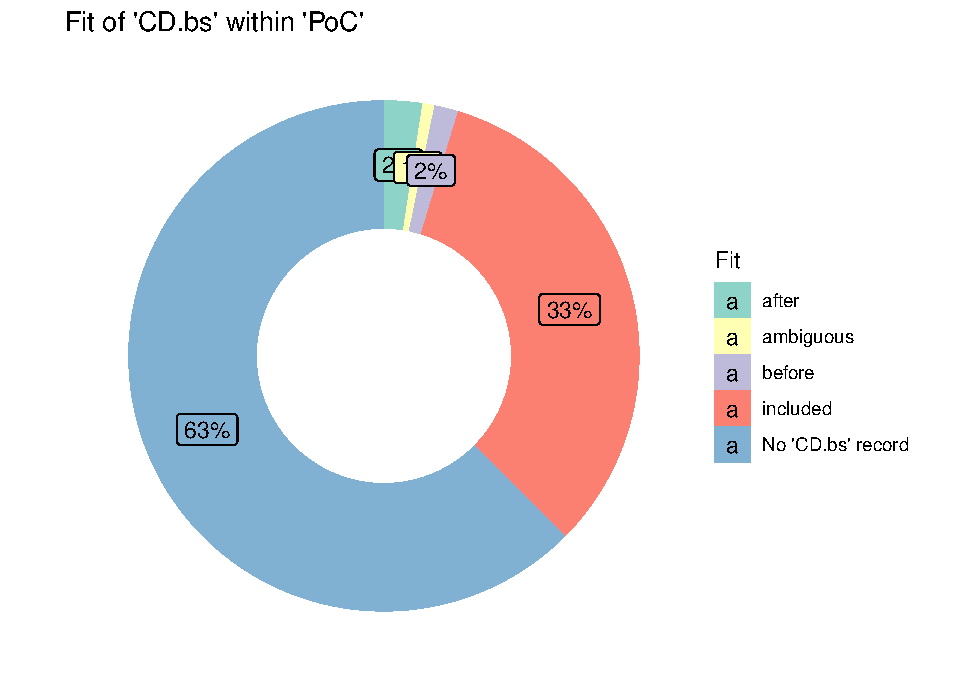
\includegraphics{Usage_code_files/figure-latex/unnamed-chunk-15-3.pdf}

\begin{itemize}
\tightlist
\item
  Summary: The building footprint area is 2279 ha.

  \begin{tabular}[t]{l|r|r}
  \hline
  PoC.source\_name & sum\_area & sum\_area\_rel\\
  \hline
  CD.abam\_1920,
  ABAM\_1920 & 1,665 & 73\\
  \hline
  CD.bs,
  BS\_1920s & 94 & 4\\
  \hline
  TP\_pub.date\_year,
  ABSM & 520 & 23\\
  \hline
  \end{tabular}
\item
  Summary: The building footprint area is 2279 ha.

  \begin{tabular}[t]{l|r|r}
  \hline
  category & sum\_area & sum\_area\_real\\
  \hline
  after & 56 & 2\\
  \hline
  ambiguous & 17 & 1\\
  \hline
  before & 35 & 2\\
  \hline
  included & 746 & 33\\
  \hline
  No 'CD.bs' record & 1,425 & 63\\
  \hline
  \end{tabular}
\item
  Summary: This table is based on data entries that have ``PoC'' and
  ``CD.bs'' records. In other words, blank ``CD.bs'' records are
  excluded. The building footprint area is 854 ha, which is 37\% of the
  total area.

  \begin{tabular}[t]{l|r|r}
  \hline
  CD.bs\_fit & sum\_area & sum\_area\_rel\\
  \hline
  after & 56 & 7\\
  \hline
  ambiguous & 17 & 2\\
  \hline
  before & 35 & 4\\
  \hline
  included & 746 & 87\\
  \hline
  \end{tabular}
\end{itemize}

\hypertarget{annnex}{%
\section*{Annnex}\label{annnex}}
\addcontentsline{toc}{section}{Annnex}

\hypertarget{write-csv-file}{%
\subsection*{Write CSV file}\label{write-csv-file}}
\addcontentsline{toc}{subsection}{Write CSV file}

\hypertarget{plotting-figures}{%
\subsection*{Plotting figures}\label{plotting-figures}}
\addcontentsline{toc}{subsection}{Plotting figures}

The figures are published in the corresponding paper.

\begin{verbatim}
## Warning: Removed 2 rows containing missing values (geom_bar).
\end{verbatim}

\begin{verbatim}
## Warning: Removed 2 rows containing missing values (geom_text).
\end{verbatim}

\end{document}
